% Chapter5

\chapter{实证分析}

\section{因子模型}\label{sfactor}
本文依据错误定价因子$M$的预测结果,构建了Q1和Q5两组的多空组合,以月度平均收益$mean$和风险调节收益$\alpha$作为绩效衡量指标。 为了避免A股市场做空机制的限制,本文还构建了Q1到Q5五组的多头组合,如果从Q1组到Q5组、从最被高估到最被低估的股票能够呈现超额收益的递增趋势,同样能证明错误定价因子$M$的有效性。

对于因子的选择,使用了常见的CAPM模型、Fama−French 三因子模型、 Carhart 四因子模型、Fama−French 五因子模型、以及Hou-Xue-Zhang 四因子模型(后称为q-因子模型),采用了其中的6组因子(CAPM、FF3、FFC、FF5、FF5+MOM、Q)进行研究,具体结果见表~\ref{factor}所示,记录了Q1到Q5五组多头组合和多空组合的月度平均收益$mean$、风险调节收益$\alpha$及$t$值。

\begin{table}[htbp]
\caption{因子模型回归}
\label{factor}
\begin{tabular*}{\hsize}{@{\hskip\tabcolsep\extracolsep\fill}*{8}{c}}
\toprule
模型                       & 系数                    & Q1 & Q2 & Q3 & Q4 & Q5 & Q5-Q1 \\ \midrule
 &$ mean$& -0.180&  0.037&0.255&0.421& 0.955&  1.135\\
 \multirow{2}{*}{CAPM}     & $\alpha$ &    0.0452         &    0.235&    0.540&    0.708&    1.153&   1.123\\
                         &$ t$值                     &     (0.52)         &   (2.71)         &   (6.24)         &   (7.80)         &   (8.26)  & (2.35)         \\
\multirow{2}{*}{FF3}     & $\alpha$ &      0.0793         &    0.271&    0.573&    0.747&    1.196&  1.096\\
                         & $t$值                     &    (0.93)         &   (3.18)         &   (6.72)         &   (8.39)         &   (8.65)      &(2.43)     \\
\multirow{2}{*}{FFC}     & $\alpha$  &  0.146  &    0.320&    0.643&    0.823&    1.268 & 1.099\\
                         &$ t$ 值                   &    (1.70)         &   (3.74)         &   (7.52)         &   (9.22)         &   (9.13)    &(2.40)       \\
\multirow{2}{*}{FF5}     &$\alpha$  & -1.186&   -1.172&   -0.941&   -0.762&   -0.143      & 0.981\\
                         & $t$  值                   &   (-9.02)         & (-12.90)         &  (-9.76)         &  (-9.01)         &  (-2.82)   &   (1.76)      \\
\multirow{2}{*}{FF5+mom} &$\alpha$  & -1.122&   -1.116&   -0.869&   -0.687&  -0.0727  &  0.984    \\
                         &$ t $ 值        &        (-11.14)         & (-11.12)         &  (-8.69)         &  (-6.56)         &  (-0.44)  & (1.75)  \\
\multirow{2}{*}{Q}       &$\alpha$  &   0.177&    0.380&    0.677&    0.853&    1.298    &1.106\\
                         & $t$   值                  &     (2.08)         &   (4.46)         &   (7.95)         &   (9.58)         &   (9.37)  &(2.43)     \\ \bottomrule
\end{tabular*}
\end{table}

可以看出在运用BRTs模型进行数据模拟后,Q1到Q5的多头组合月度平均收益$mean$、风险调节收益$\alpha$均呈现递增趋势,并且非常显著;Q1、Q5的多空组合也有显著的正收益,证明了错误定价因子$M$的作用,以及基本面分析的有效性。

附录~\ref{linear}~展现了采用线性回归方法的因子模型结果,可以看出结果也非常显著,佐证了本文的结论。
但相比而言,采用BRTs算法得到的Q1、Q5的多空组合收益率更高;
并且BRTs算法能够有效处理缺失值的问题,而线性回归对于缺失值非常敏感,数据量大大缩水,虽然两种方法结果相似,但对于结果或多或少仍有影响,如果扩展到其他研究中,这种数据的直接丢弃或许是致命的。

\section{Fama-MacBeth截面回归}\label{sfmb}
表~\ref{fmb}~展现了对于所有公司Fama-MacBeth的时间序列截面回归结果,两列分别选用了不同的控制变量来表现错误定价因子M的预测能力,所有列均控制了行业固定效应,括号内的数字代表$t$值。

其中,第一列仅采用了$M$作为解释变量,结果非常显著;第二列新加入了公司特征作为控制变量:$beta$值、市净率$BM$、三个动量因子$lagretn$、$mom12$、$mom36$、市盈率$EP$、净经营性资产增长率$grltnoa$与毛利率$PA$,让回归更为完整,错误定价因子$M$同样显著,说明错误定价因子$M$可以用来预测股票未来收益。

\begin{table}[htbp]\centering
\def\sym#1{\ifmmode^{#1}\else\(^{#1}\)\fi}
\caption{Fama-MacBeth截面回归}
\label{fmb}
\begin{tabular*}{0.85\hsize}{@{\hskip\tabcolsep\extracolsep\fill}*{3}{c}}
\toprule
        &\multicolumn{1}{c}{(1)}&\multicolumn{1}{c}{(2)}\\
 &\multicolumn{1}{c}{$R_{t+1}$}&\multicolumn{1}{c}{$R_{t+1}$}\\
\midrule
$M$         &    1.623\sym{***}&    6.601\sym{**} \\
          &  (10.82)         &   (1.98)         \\
$beta  $    &                  &    20.08\sym{***}\\
          &                  &   (8.23)         \\
$BM  $      &                  &    27.61         \\
          &                  &   (1.48)         \\
$EP  $      &                  &   -252.2         \\
          &                  &  (-0.52)         \\
$lagretn $  &                  &   -13.03\sym{***}\\
          &                  &  (-3.39)         \\
$mom12  $   &                  &    8.121\sym{***}\\
          &                  &   (5.43)         \\
$mom36  $   &                  &    3.545\sym{**} \\
          &                  &   (2.42)         \\
$grltnoa $  &                  &   -0.757         \\
          &                  &  (-0.17)         \\
$PA   $     &                  &   -176.7\sym{*}  \\
          &                  &  (-1.80)         \\
行业固定效应&    控制   &    控制   \\
\midrule
$N$         &   129169         &    50153     \\
$R^2$        &   0.0557         &    0.572     \\
\bottomrule
\multicolumn{3}{l}{\footnotesize \textit{t} statistics in parentheses}\\
\multicolumn{3}{l}{\footnotesize \sym{*} \(p<0.1\), \sym{**} \(p<0.05\), \sym{***} \(p<0.01\)}\\
\end{tabular*}
\end{table}

\section{股票特征重要性}
如图~\ref{feature}~所示,在对公司内在价值的回归计算过程中,对51个财务指标进行重要性排序。其中,$y$轴显示了所有财务指标,$x$轴代表了不同财务指标的重要性比例,可见最为重要的指标有股本、净利润,分别占到了约10\%、6\%,对应说明评估公司内在价值的重要因素一般在于股东行为以及公司业务的利润大小等。

\begin{figure}[htbp]
  \centering
    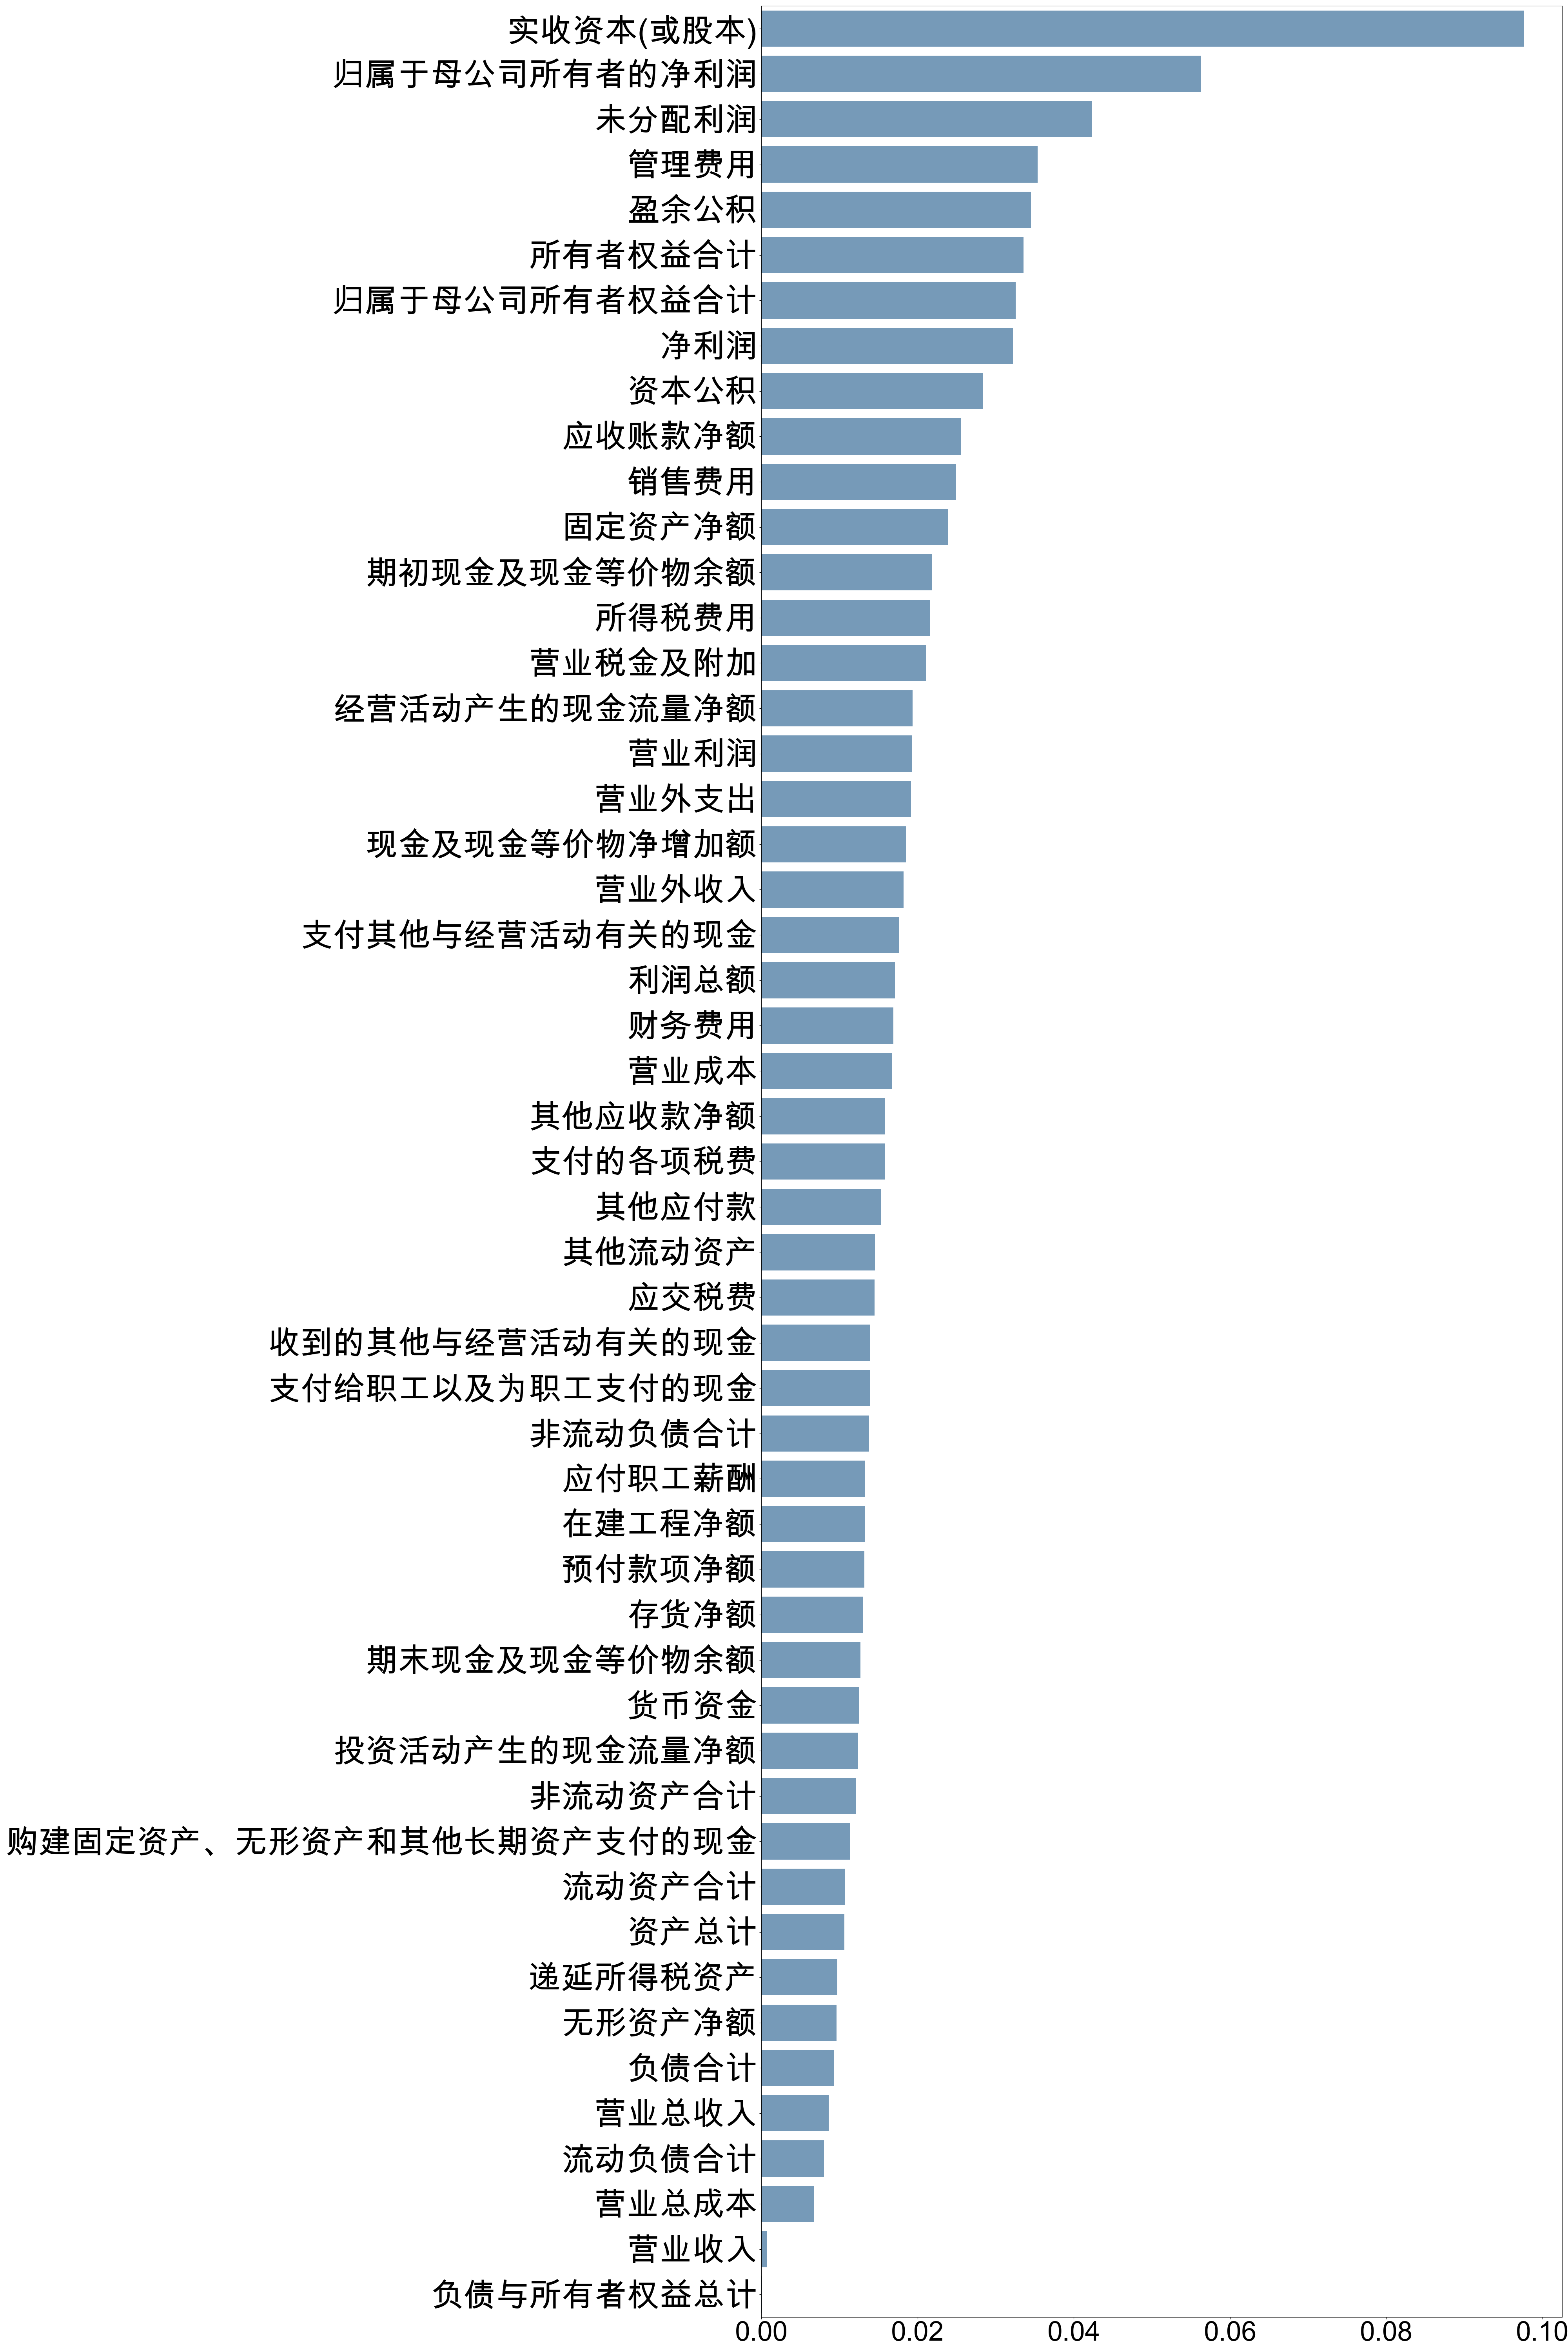
\includegraphics[width=\linewidth]{feature importance1.png}
    \caption{股票特征重要性}
    \label{feature}
\end{figure}

\section{稳健性分析}
上述小节~\ref{sfmb}、\ref{sfactor}~的结果证明了错误定价因子$M$以及基本面分析的有效性,公司内在价值能够完全反映于财务指标。为检验超额利润是否真正来自于错误定价而非因子遗漏,即市场价值是否会逐渐趋向于内在价值,本文进行以下稳健性分析。

在第$t$期计算各公司的错误定价因子$M$,并分为Q1到Q5五组,构建Q1与Q5两组的多空组合,基于该投资组合计算未来36期的收益情况,同上文采用六组因子(CAPM、FF3、FFC、FF5、FF5+MOM、Q)进行研究,结果如图~\ref{signal1}、\ref{signal2}、\ref{signal3}、\ref{signal4}、\ref{signal5}、\ref{signal6}~所示。

\begin{figure}[htbp]
  \centering
    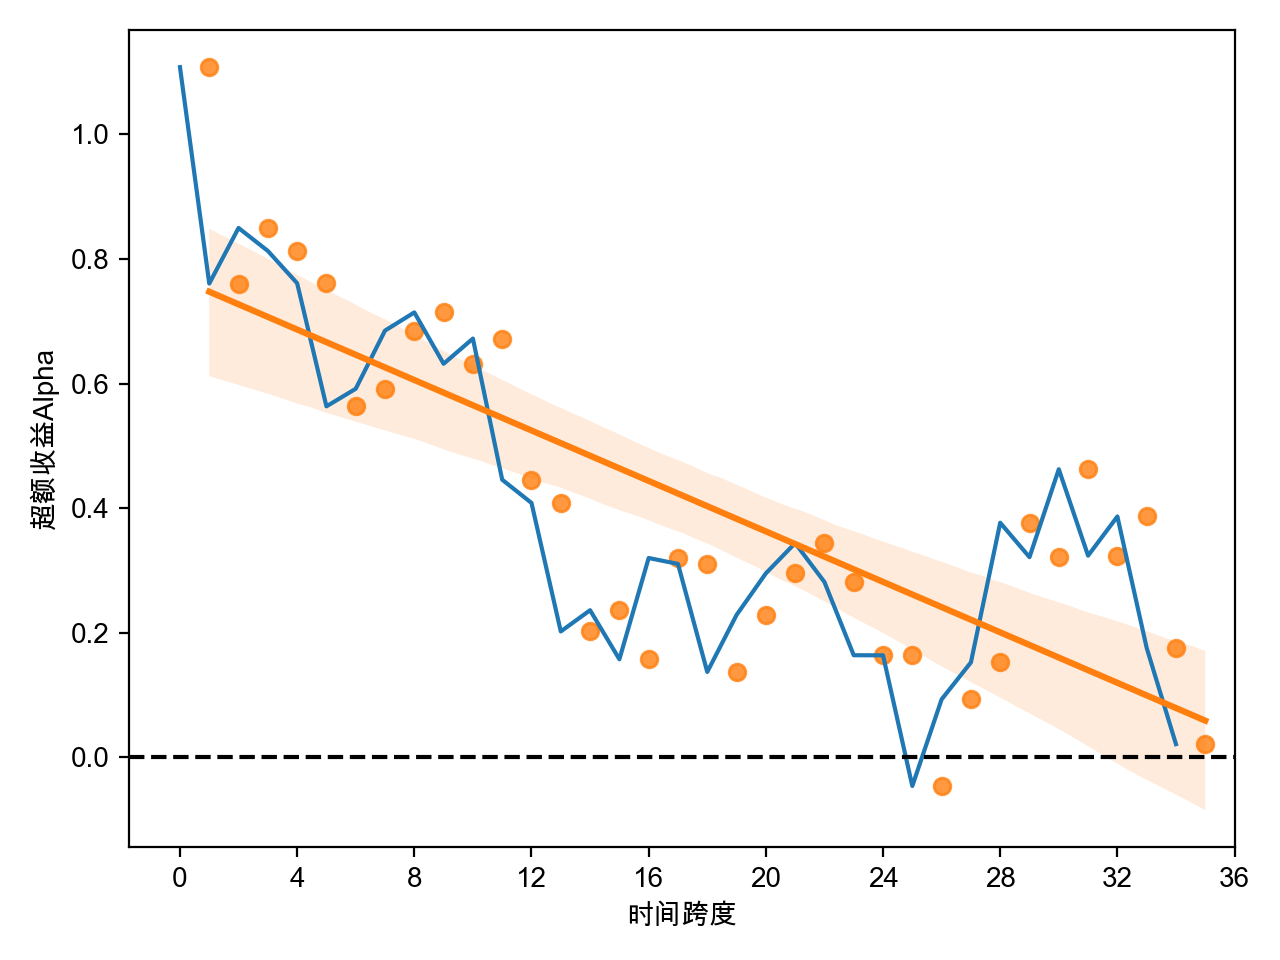
\includegraphics[width=\linewidth]{signal delay1.png}
    \caption{信号延迟(CAPM模型)}
    \label{signal1}
\end{figure}
     
\begin{figure}[htbp]
  \centering
    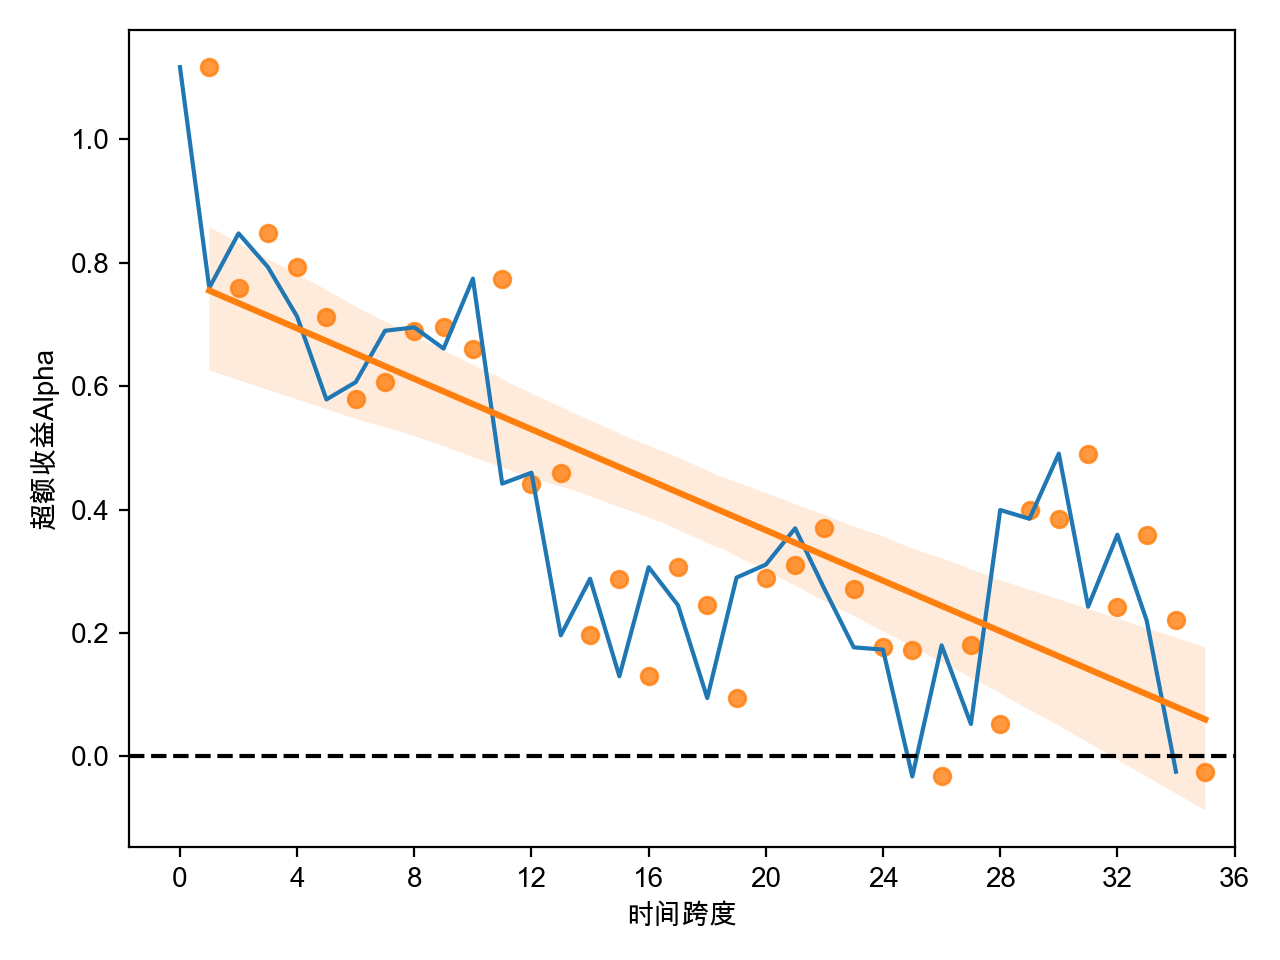
\includegraphics[width=\linewidth]{signal delay2.png}
    \caption{信号延迟(FF3模型)}
    \label{signal2}
\end{figure}

\begin{figure}[htbp]
  \centering
    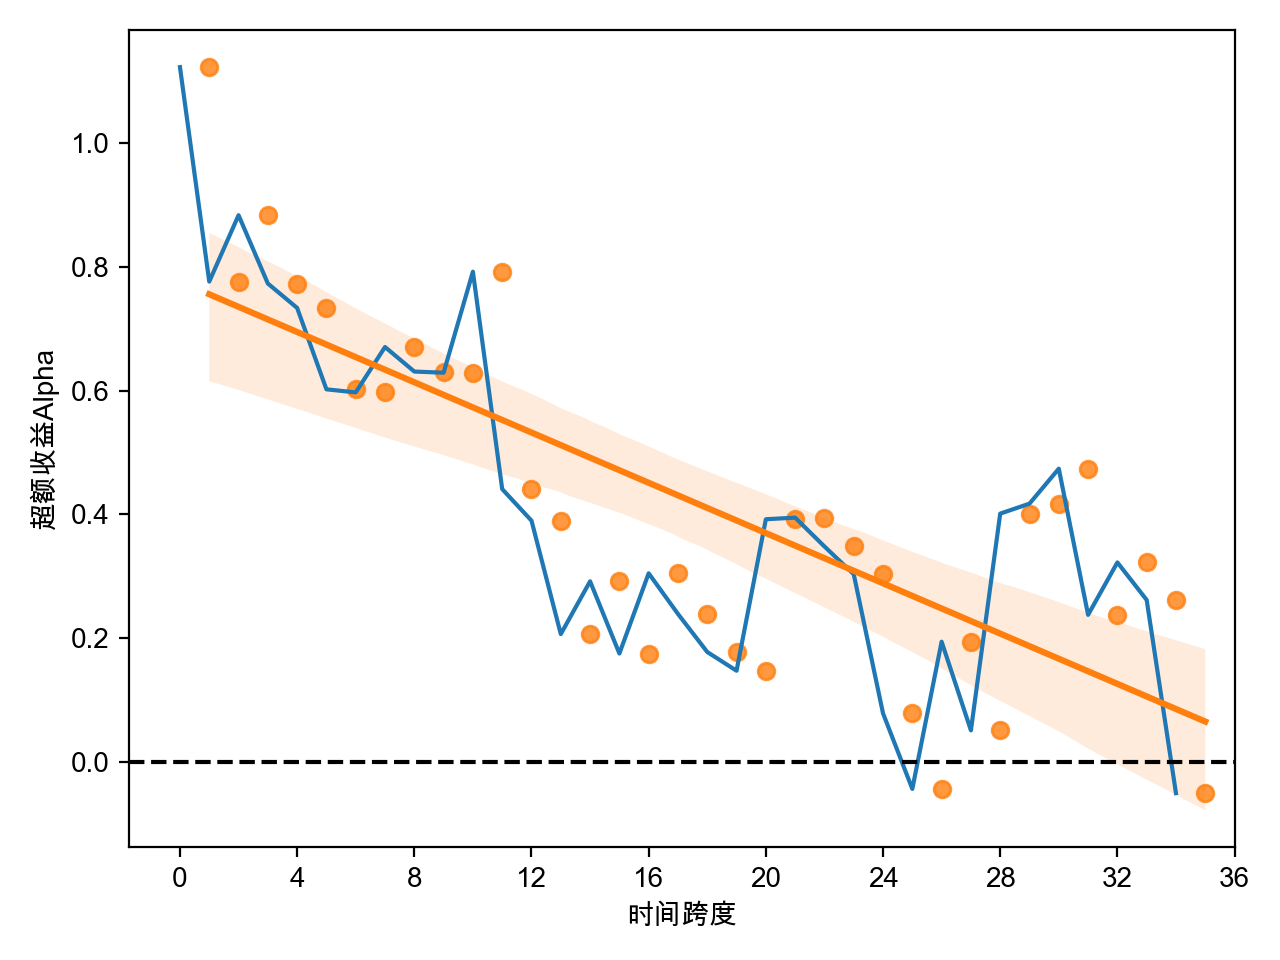
\includegraphics[width=\linewidth]{signal delay3.png}
    \caption{信号延迟(FFC模型)}
    \label{signal3}
\end{figure}
  
\begin{figure}[htbp]
  \centering
    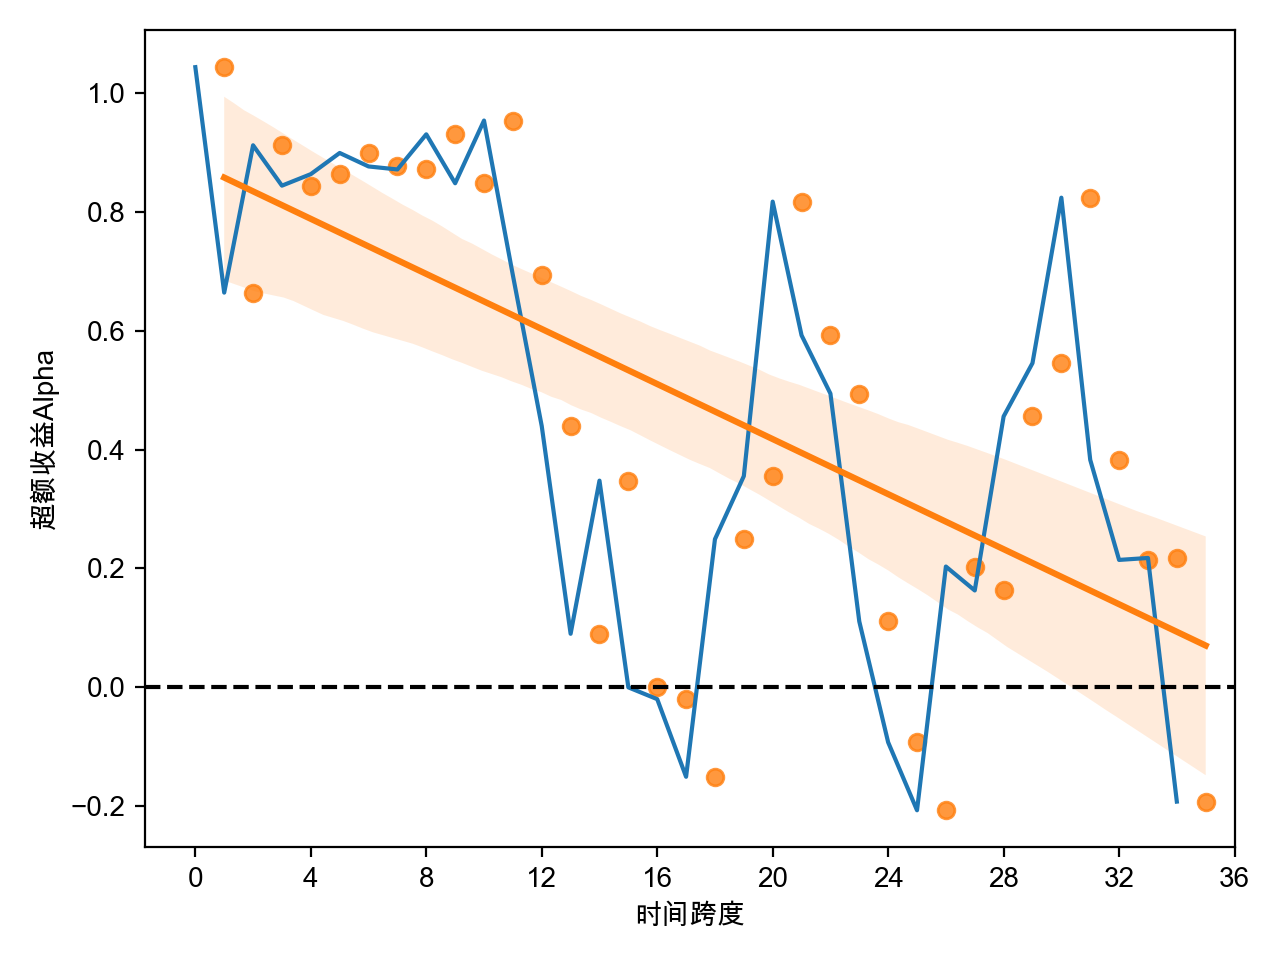
\includegraphics[width=\linewidth]{signal delay4.png}
    \caption{信号延迟(FF5模型)}
    \label{signal4}
\end{figure}

\begin{figure}[htbp]
  \centering
    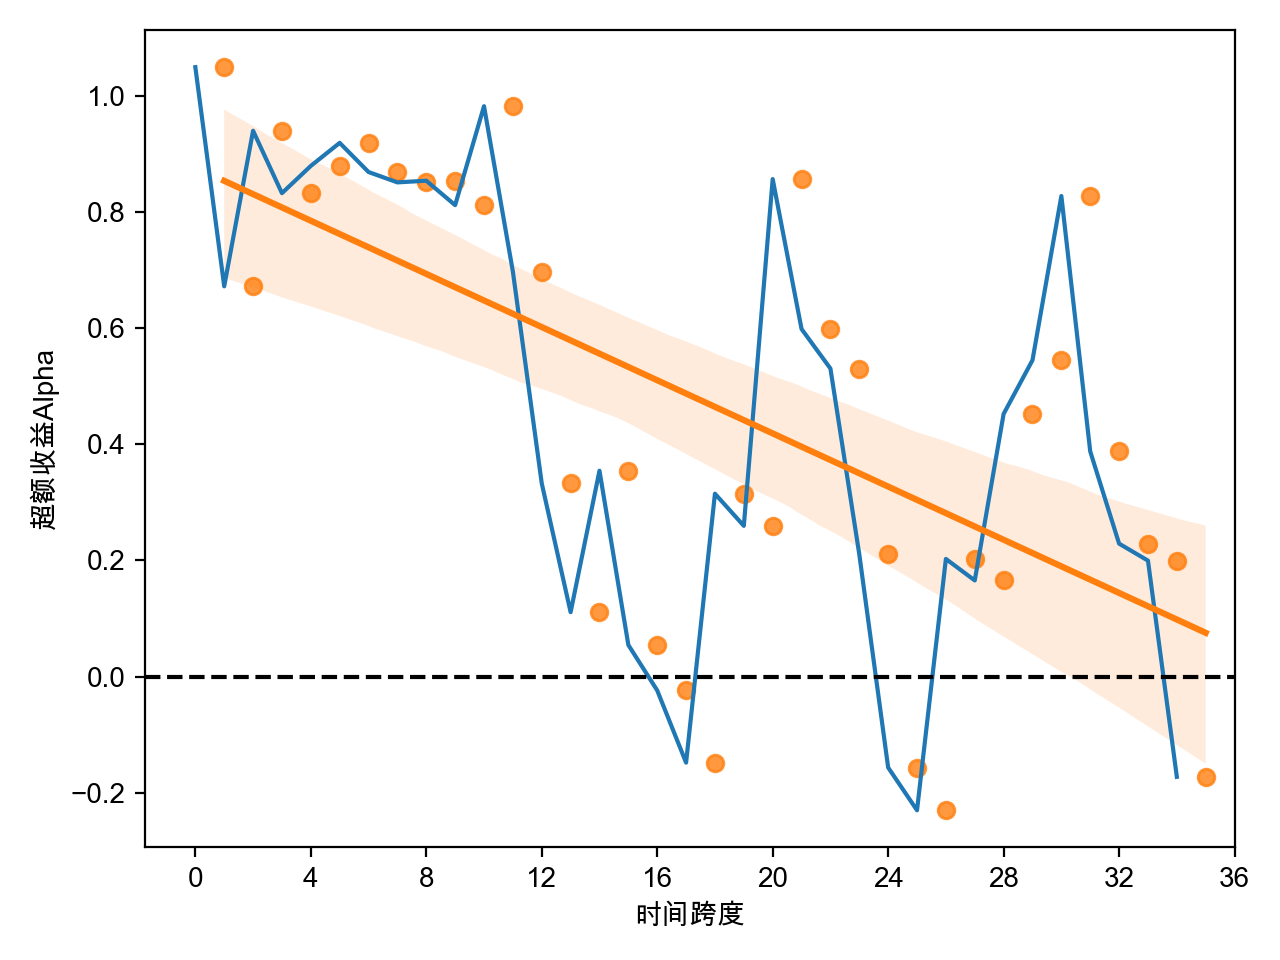
\includegraphics[width=\linewidth]{signal delay5.png}
    \caption{信号延迟(FF5+MOM模型)}
    \label{signal5}
\end{figure}
  
\begin{figure}[htbp]
  \centering
    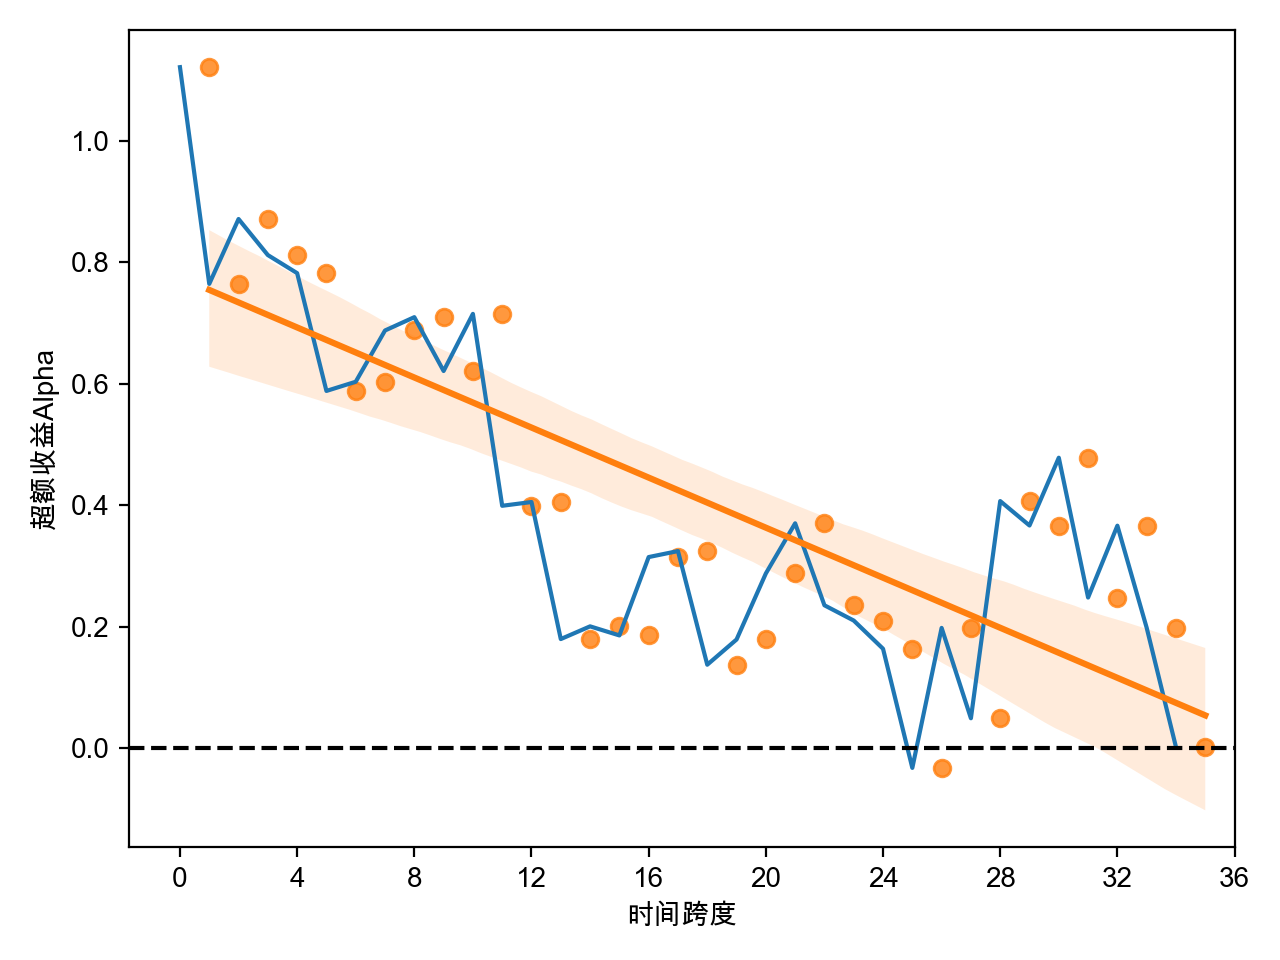
\includegraphics[width=\linewidth]{signal delay6.png}
    \caption{信号延迟(Q因子模型)}
    \label{signal6}
\end{figure}

在六组模型中,多空组合收益均在当前第$t$期拥有最高的超额收益$\alpha$,但后面随着时间增长,收益呈现明显的下降趋势,说明当前时点的错误定价已经随着时间而抵消,股票的市场价格能够灵活随着信息进行调整,进而逐渐趋近于内在价值,收益也就越来越小,证明了本文在每一期重新进行内在价值计算、根据错误定价因子$M$对公司进行分组的正确性。若采用过往时点的结果进行未来股票收益的分析,会产生一定的偏误,所以对于运用错误定价因子$M$进行投资组合的构建,要做到及时更新。

\begin{figure}[htbp]
  \centering
    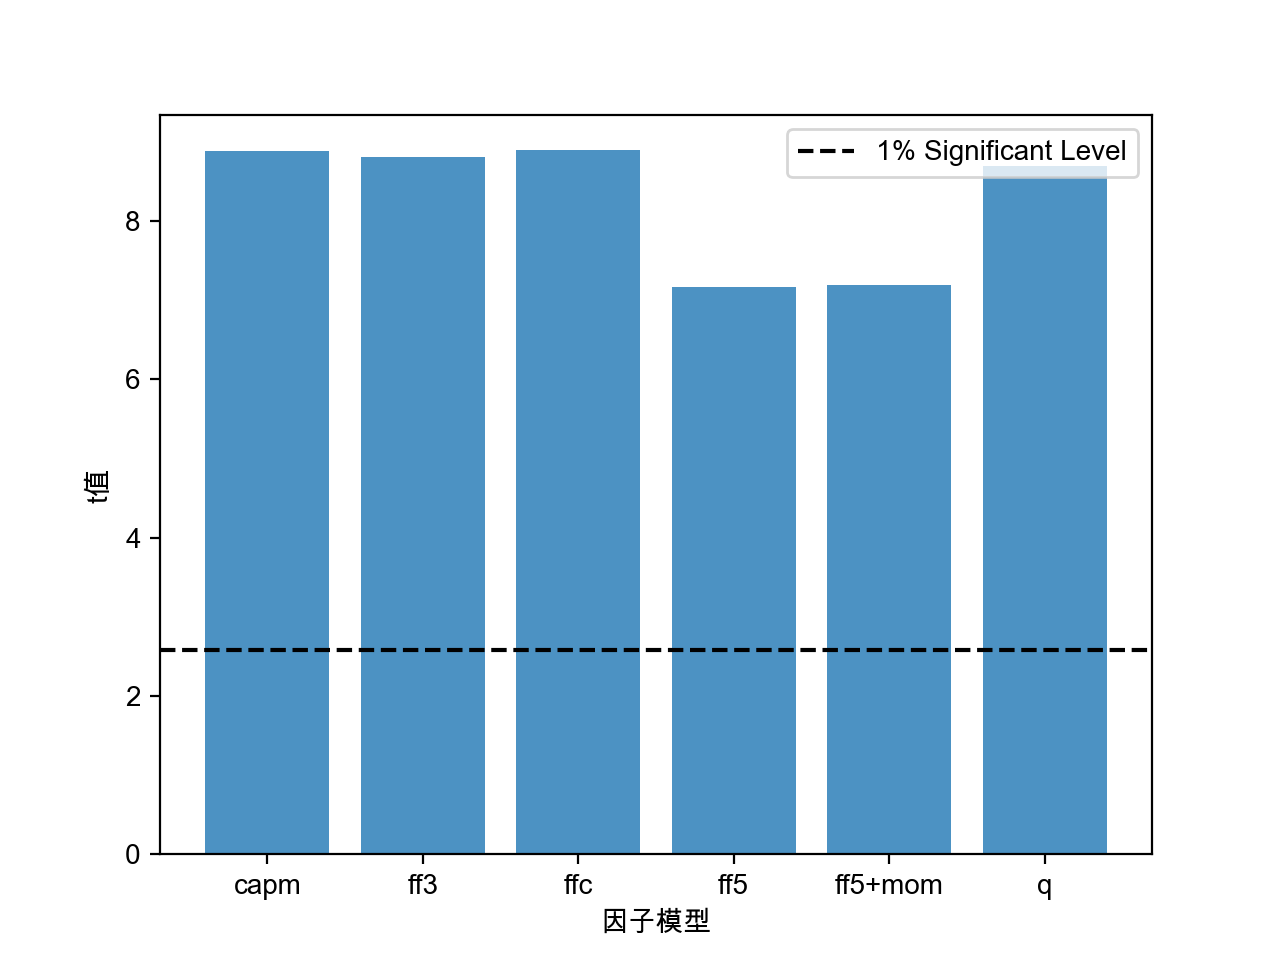
\includegraphics[width=\linewidth]{t_value.png}
      \caption{五组模型多空组合显著性检验}
    \label{t}
\end{figure}

图~\ref{t}~是对于六组因子模型中多空组合收益是否显著大于0的检验,所有模型结果均在1\%的显著性水平下成立,证明了运用财务指标衡量公司内在价值的可行性、根据错误定价因子$M$进行公司分组的有效性。


